\documentclass[letter]{scrartcl}
\usepackage{graphicx}
\usepackage{fullpage} %1in margins
\usepackage{tabularx}
\usepackage{hyperref}
\usepackage{tikz} % for diagrams
\usetikzlibrary{automata,positioning}

\newcommand{\app}{\sc{393torrent}}

\begin{document}

\title{Requirements for \app}
\subtitle{Dan Keller, Kenneth Link, Nathan McKinley, Ross Nanopoulos}
\date{} % no date

\maketitle

\begin{abstract}
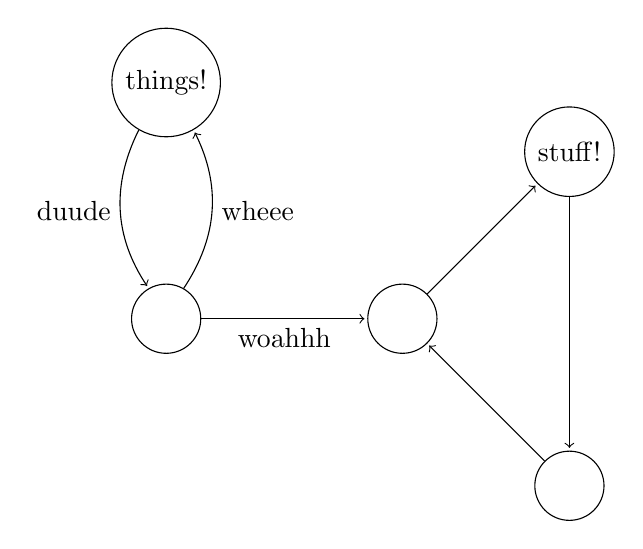
\begin{tikzpicture}[shorten >=1pt,node distance=3cm,on grid,auto]
	\node[state] (s) {};
	\node[state] (a1) [above=of s] {things!};
	\node[state] (b1) [right=of s] {};
	\node[state] (b2) [above right=of b1] {stuff!};
	\node[state] (b3) [below right=of b1] {};
	\path[->]
	(s)  edge [bend right] node [right] {wheee} (a1)
	     edge node [below] {woahhh} (b1)
	(a1) edge [bend right] node [left] {duude} (s)
	(b1) edge node {} (b2)
	(b2) edge node {} (b3)
	(b3) edge node {} (b1);
\end{tikzpicture}

The software requirements specification (SRS) specifies all user stories (i.e. functional requirements) as well as nonfunctional requirements. These requirements are used in iteration planning as well as acceptance testing.  This document should be used by the members of the 393torrent team, who will implement and verify the functionality of the BitTorrent client.
\end{abstract}

\tableofcontents
\pagebreak

\section{Overview}
The BitTorrent client (393torrent) will allow users to download, create, and seed torrent files.  It will enable them to achieve the full functionality of a BitTorrent client in a lightweight form.  The primary objective of this BitTorrent client is to offer a free and open source alternative--without advertisements--to the current heavyweight clients available.  Specific goals of 393torrent can be found in the vision and scope document.

\section{Protocol}

\section{App Architecture}

\section{Thread Model}

\section{Classes in Detail}

\pagebreak
\section{Author Contributions}
This section provides the details to what each author contributed to the vision and scope document, as requested per professor Podgurski.
\subsection{Daniel Keller}
Created document outline and 
\subsection{Kenneth Link}

\subsection{Nathan McKinley}

\subsection{Ross Nanopoulos}


\section{Inspection}
\begin{tabularx}{\textwidth}{X c c}
\textbf{Comment} & \textbf{Reported By} & \textbf{Fixed By} \\
\end{tabularx}
\end{document}
